\documentclass[13pt, a4paper, twoside]{mwart}
\usepackage[a4paper]{geometry}
\geometry{left=3cm}
\geometry{right=1.5cm}
\geometry{top=2cm}
\geometry{bottom=1.5cm}
\usepackage[pdftex]{graphicx}
\graphicspath{{img/}}

\usepackage[utf8]{inputenc}
\usepackage{polski}
\usepackage[polish]{babel}
\usepackage{tabularx}
\usepackage{datetime}
\usepackage{listings}
\usepackage{courier}
\lstset{basicstyle=\footnotesize}

\newcommand{\coursename}{Modelowanie i Analiza Systemów}
\newcommand{\labnumber}{1}
\newcommand{\labname}{Generator sygnałów testujących i prosty układ kombinacyjny}
\newcommand{\studentname}{Maciej Stanek}
\newcommand{\studentnumber}{122352}
\newdate{labdate}{9}{3}{2018}
\newdate{labreportdate}{30}{3}{2018}

\usepackage{fancyhdr}
\pagestyle{fancy}
\fancyhead[RO,LE]{\thepage}
\fancyhead[LO]{\textbf{LAB\#\labnumber} \labname}
\fancyhead[RE]{\coursename}
\fancyfoot{}

\begin{document}

\begin{center}
  \textbf{\LARGE{Sprawozdanie z laboratorium}}
\end{center}

\noindent
\begin{tabularx}{\linewidth}{rX}
  \textbf{Przedmiot} & \coursename \\
  \textbf{Temat laboratorium} & \labname \\
  \textbf{Numer laboratorium} & \labnumber \\
  \textbf{Imię i nazwisko} & \studentname \\
  \textbf{Numer indeksu} & \studentnumber \\
  \textbf{Data wykonania} & \displaydate{labdate} \\
  \textbf{Data sprawozdania} & \displaydate{labreportdate} \\
\end{tabularx}

\vspace{0.3cm}
\noindent\hrulefill

%%%%%%%%%%%%%%%%%%%%%%%%%%%%%%%%%%%%%%%%%%%%%%%%%%%%%%%%%%%%%%%%%%%%%%%%%%%%%%%

\lstinputlisting[
  language=VHDL,
  caption={Implementacja generatora z zadania pierwszego wraz z pustą architekturą}
  ]{../lab1/gen.vhd}

\lstinputlisting[
  language=tcl,
  caption={Skrypt testujący generator z zadania drugiego}
  ]{../lab1/gen.do}

\begin{figure}[h]
	\centering
	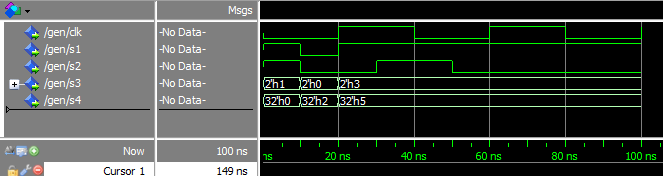
\includegraphics[width=\linewidth]{1.png}
	\caption{Wyniki symulacji generatorów z zadania pierwszego i drugiego.}
\end{figure}

\begin{figure}[h]
	\centering
	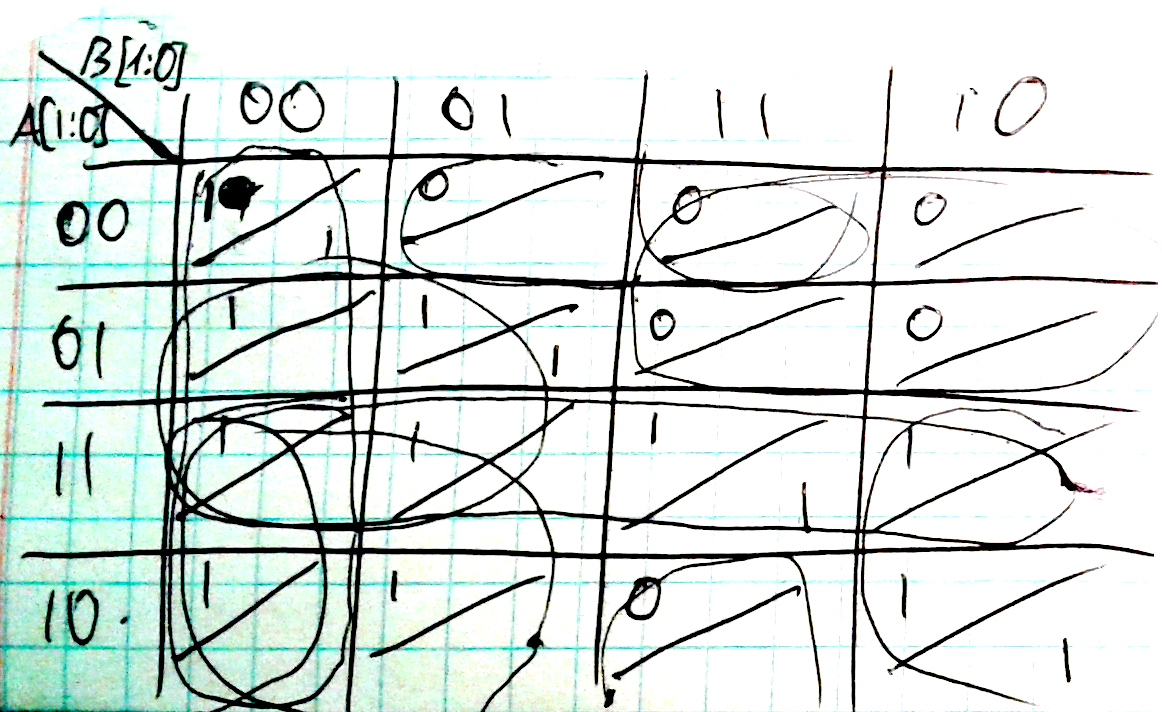
\includegraphics[width=0.4\linewidth]{karnaugh.png}
	\caption{Tablica Karnaugh dla wyjść EQ i GE}
\end{figure}

\begin{figure}[h]
	\centering
	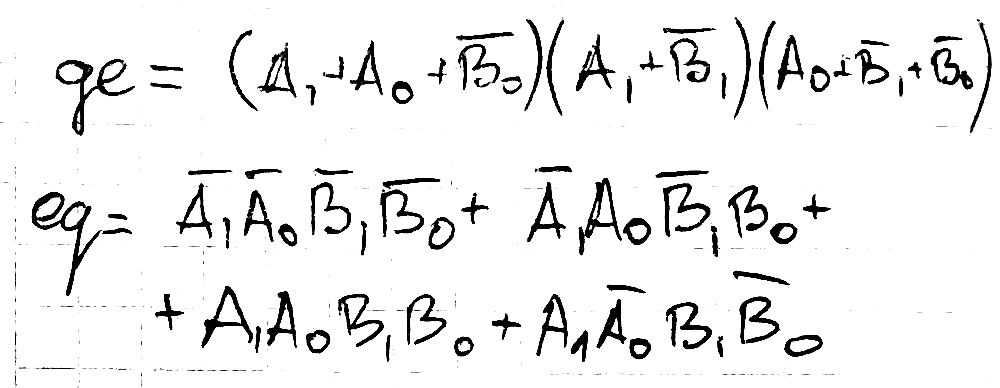
\includegraphics[width=0.4\linewidth]{geeq.png}
	\caption{Równania wyjść EQ i GE wyznaczone na podstawie tablicy Karnaugh}
\end{figure}

\lstinputlisting[
  language=VHDL,
  caption={Implementacja sumatora w architekturach behawioralnej i strukturalnej}
  ]{../lab1/uklad_kombinacyjny_porownujacy_dwie_liczby_dwubitowe.vhd}

\lstinputlisting[
  language=tcl,
  caption={Skrypt testujący sumator z zadania trzeciego}
  ]{../lab1/uklad_kombinacyjny_porownujacy_dwie_liczby_dwubitowe.do}

\begin{figure}[h]
	\centering
	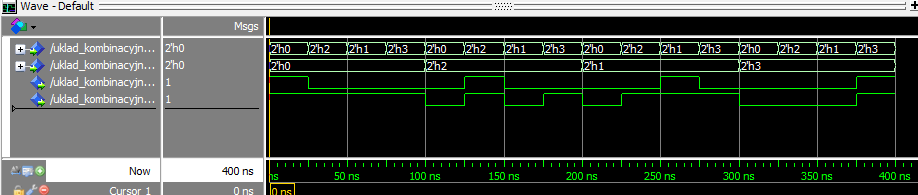
\includegraphics[width=\linewidth]{compare_structural.png}
  \caption{Wynik działania architektury strukturalnej}
\end{figure}

\begin{figure}[h]
	\centering
	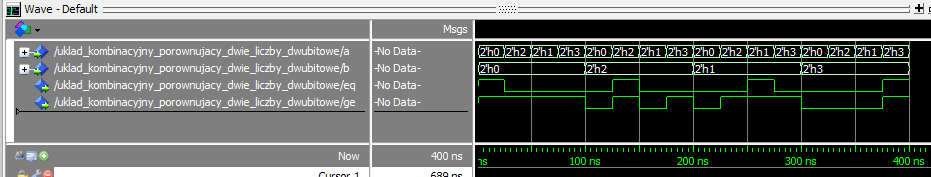
\includegraphics[width=\linewidth]{compare_behavioral.png}
  \caption{Wynik działania architektury behawioralnej}
\end{figure}

%%%%%%%%%%%%%%%%%%%%%%%%%%%%%%%%%%%%%%%%%%%%%%%%%%%%%%%%%%%%%%%%%%%%%%%%%%%%%%%

\end{document}
